
\large
\part{Fundamentals of AE}


\section{Introduction}

Acoustic Emission is kind of non-destructive passive testing, where the
signal is detected by surface-mounted piezoelectric sensors as opposed
to ultrasonic active testing where the signals are emitted through the
specimen and transmitted back. To acquire such signals, the component
under test is submitted to external stimuli, such as loads , high
pressure, or relatively high temperature. As the damage grows through
the component, more energy is released in the process. This kind of
testing is generally used for evaluating the structural integrity of
certain component to monitor defects like fatigue cracking, fiber break,
and corrosion progression through the material. Also, being
non-destructive, AE testing allows large structures to be monitored
while they are operating causing minimal disruption.

\section{Signal Parameters}

Analysis of AE data is quite difficult as the number of data point
produced from a single test is large. So Extracting features from the
waveform allows comparisons between different set of data.

\textbf{Amplitude:} is the maximum measured voltage across the
waveform. It is an important parameter as it determines the parts of the
wave which will not be included in the analysis (some points do not
cross the threshold defined based on the value of the amplitude).

\textbf{Time of arrival :} regarded as the most import feature in the
waveform. ToA determines the time that sensor began to sense the wave
coming form the AE event. They are some method to compute ToA, like
threshold crossing and Akaike information criterion (AIC), but they will
be discussed in detail later.

There are some other important signal parameters like: rise time ,
counts , duration; however, they are irrelevant to the scope of this
project.

\section{Data Acquisition Setup}

The setup is quite easy, just four sensors placed on a known size grid.
When the hit takes place each of the sensor sends its received signal to
the corresponding channels to be filtered as some noise might interfere.
After that the signal get recorded by a specialized acquisition software
to be further exported to CSV files , for example. This short journey
can be summarized by the following figure.

    \begin{figure}[htbp]
        \centering
        \scalebox{0.9}{


\tikzset{every picture/.style={line width=0.75pt}} %set default line width to 0.75pt        

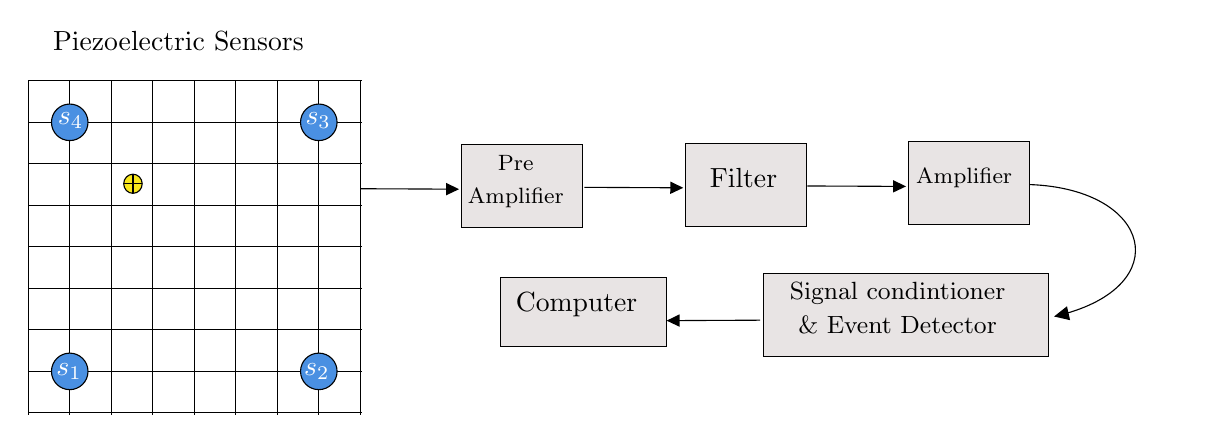
\begin{tikzpicture}[x=0.75pt,y=0.75pt,yscale=-1,xscale=1]
%uncomment if require: \path (0,300); %set diagram left start at 0, and has height of 300

%Shape: Grid [id:dp18492571195627683] 
\draw  [draw opacity=0] (42,46) -- (202.61,46) -- (202.61,207) -- (42,207) -- cycle ; \draw   (42,46) -- (42,207)(62,46) -- (62,207)(82,46) -- (82,207)(102,46) -- (102,207)(122,46) -- (122,207)(142,46) -- (142,207)(162,46) -- (162,207)(182,46) -- (182,207)(202,46) -- (202,207) ; \draw   (42,46) -- (202.61,46)(42,66) -- (202.61,66)(42,86) -- (202.61,86)(42,106) -- (202.61,106)(42,126) -- (202.61,126)(42,146) -- (202.61,146)(42,166) -- (202.61,166)(42,186) -- (202.61,186)(42,206) -- (202.61,206) ; \draw    ;
%Shape: Circle [id:dp2888619155752197] 
\draw  [color={rgb, 255:red, 0; green, 0; blue, 0 }  ,draw opacity=1 ][fill={rgb, 255:red, 74; green, 144; blue, 226 }  ,fill opacity=1 ] (53.2,66) .. controls (53.2,61.14) and (57.14,57.2) .. (62,57.2) .. controls (66.86,57.2) and (70.8,61.14) .. (70.8,66) .. controls (70.8,70.86) and (66.86,74.8) .. (62,74.8) .. controls (57.14,74.8) and (53.2,70.86) .. (53.2,66) -- cycle ;
%Shape: Circle [id:dp6470369433137191] 
\draw  [color={rgb, 255:red, 0; green, 0; blue, 0 }  ,draw opacity=1 ][fill={rgb, 255:red, 74; green, 144; blue, 226 }  ,fill opacity=1 ] (173.2,66) .. controls (173.2,61.14) and (177.14,57.2) .. (182,57.2) .. controls (186.86,57.2) and (190.8,61.14) .. (190.8,66) .. controls (190.8,70.86) and (186.86,74.8) .. (182,74.8) .. controls (177.14,74.8) and (173.2,70.86) .. (173.2,66) -- cycle ;
%Shape: Circle [id:dp7811582779529831] 
\draw  [color={rgb, 255:red, 0; green, 0; blue, 0 }  ,draw opacity=1 ][fill={rgb, 255:red, 74; green, 144; blue, 226 }  ,fill opacity=1 ] (53.2,186) .. controls (53.2,181.14) and (57.14,177.2) .. (62,177.2) .. controls (66.86,177.2) and (70.8,181.14) .. (70.8,186) .. controls (70.8,190.86) and (66.86,194.8) .. (62,194.8) .. controls (57.14,194.8) and (53.2,190.86) .. (53.2,186) -- cycle ;
%Shape: Circle [id:dp09864792938797584] 
\draw  [color={rgb, 255:red, 0; green, 0; blue, 0 }  ,draw opacity=1 ][fill={rgb, 255:red, 74; green, 144; blue, 226 }  ,fill opacity=1 ] (173.2,186) .. controls (173.2,181.14) and (177.14,177.2) .. (182,177.2) .. controls (186.86,177.2) and (190.8,181.14) .. (190.8,186) .. controls (190.8,190.86) and (186.86,194.8) .. (182,194.8) .. controls (177.14,194.8) and (173.2,190.86) .. (173.2,186) -- cycle ;
%Shape: Rectangle [id:dp1276758359868515] 
\draw  [fill={rgb, 255:red, 232; green, 228; blue, 228 }  ,fill opacity=1 ] (250.67,76.67) -- (308.91,76.67) -- (308.91,116.67) -- (250.67,116.67) -- cycle ;
%Straight Lines [id:da18614192902932336] 
\draw    (202,98) -- (246.58,98.2) ;
\draw [shift={(249.58,98.22)}, rotate = 180.26] [fill={rgb, 255:red, 0; green, 0; blue, 0 }  ][line width=0.08]  [draw opacity=0] (6.25,-3) -- (0,0) -- (6.25,3) -- cycle    ;
%Shape: Rectangle [id:dp38520186682774127] 
\draw  [fill={rgb, 255:red, 232; green, 228; blue, 228 }  ,fill opacity=1 ] (358.67,76) -- (416.91,76) -- (416.91,116) -- (358.67,116) -- cycle ;
%Straight Lines [id:da6799885500522758] 
\draw    (310,97.33) -- (354.58,97.54) ;
\draw [shift={(357.58,97.55)}, rotate = 180.26] [fill={rgb, 255:red, 0; green, 0; blue, 0 }  ][line width=0.08]  [draw opacity=0] (6.25,-3) -- (0,0) -- (6.25,3) -- cycle    ;
%Shape: Rectangle [id:dp9128309450634404] 
\draw  [fill={rgb, 255:red, 232; green, 228; blue, 228 }  ,fill opacity=1 ] (466,75.33) -- (524.25,75.33) -- (524.25,115.33) -- (466,115.33) -- cycle ;
%Straight Lines [id:da032492736194410954] 
\draw    (417.33,96.67) -- (461.91,96.87) ;
\draw [shift={(464.91,96.88)}, rotate = 180.26] [fill={rgb, 255:red, 0; green, 0; blue, 0 }  ][line width=0.08]  [draw opacity=0] (6.25,-3) -- (0,0) -- (6.25,3) -- cycle    ;
%Shape: Rectangle [id:dp0975857174034227] 
\draw  [fill={rgb, 255:red, 232; green, 228; blue, 228 }  ,fill opacity=1 ] (396.25,138.67) -- (533.58,138.67) -- (533.58,178.67) -- (396.25,178.67) -- cycle ;
%Curve Lines [id:da709052688091981] 
\draw    (524.67,96) .. controls (583.35,98.18) and (595.23,144.79) .. (538.87,158.93) ;
\draw [shift={(536.25,159.55)}, rotate = 347.33] [fill={rgb, 255:red, 0; green, 0; blue, 0 }  ][line width=0.08]  [draw opacity=0] (7.14,-3.43) -- (0,0) -- (7.14,3.43) -- cycle    ;
%Shape: Rectangle [id:dp40604606489297823] 
\draw  [fill={rgb, 255:red, 232; green, 228; blue, 228 }  ,fill opacity=1 ] (269.33,140.67) -- (349.58,140.67) -- (349.58,174.22) -- (269.33,174.22) -- cycle ;
%Straight Lines [id:da95490291447343] 
\draw    (394.67,161.33) -- (352.58,161.54) ;
\draw [shift={(349.58,161.55)}, rotate = 359.72] [fill={rgb, 255:red, 0; green, 0; blue, 0 }  ][line width=0.08]  [draw opacity=0] (6.25,-3) -- (0,0) -- (6.25,3) -- cycle    ;
\draw  [fill={rgb, 255:red, 248; green, 231; blue, 28 }  ,fill opacity=1 ] (88,95.61) .. controls (88,93.06) and (90,91) .. (92.46,91) .. controls (94.92,91) and (96.91,93.06) .. (96.91,95.61) .. controls (96.91,98.15) and (94.92,100.22) .. (92.46,100.22) .. controls (90,100.22) and (88,98.15) .. (88,95.61) -- cycle ; \draw   (88,95.61) -- (96.91,95.61) ; \draw   (92.46,91) -- (92.46,100.22) ;

% Text Node
\draw (55,60) node [anchor=north west][inner sep=0.75pt]  [color={rgb, 255:red, 255; green, 255; blue, 255 }  ,opacity=1 ] [align=left] {$\displaystyle s_{4}$};
% Text Node
\draw (174.33,60) node [anchor=north west][inner sep=0.75pt]  [color={rgb, 255:red, 255; green, 255; blue, 255 }  ,opacity=1 ] [align=left] {$\displaystyle s_{3}$};
% Text Node
\draw (54.33,181) node [anchor=north west][inner sep=0.75pt]  [color={rgb, 255:red, 255; green, 255; blue, 255 }  ,opacity=1 ] [align=left] {$\displaystyle s_{1}$};
% Text Node
\draw (173.67,181) node [anchor=north west][inner sep=0.75pt]  [color={rgb, 255:red, 255; green, 255; blue, 255 }  ,opacity=1 ] [align=left] {$\displaystyle s_{2}$};
% Text Node
\draw (249.33,80.67) node [anchor=north west][inner sep=0.75pt]   [align=left] {\begin{minipage}[lt]{39.48pt}\setlength\topsep{0pt}
\begin{center}
{\footnotesize Pre}\\{\footnotesize Amplifier}
\end{center}

\end{minipage}};
% Text Node
\draw (366.67,86.67) node [anchor=north west][inner sep=0.75pt]   [align=left] {\begin{minipage}[lt]{27.97pt}\setlength\topsep{0pt}
\begin{center}
Filter
\end{center}

\end{minipage}};
% Text Node
\draw (465.33,86.67) node [anchor=north west][inner sep=0.75pt]   [align=left] {\begin{minipage}[lt]{39.48pt}\setlength\topsep{0pt}
\begin{center}
{\footnotesize Amplifier}
\end{center}

\end{minipage}};
% Text Node
\draw (396.67,142) node [anchor=north west][inner sep=0.75pt]   [align=left] {\begin{minipage}[lt]{94.37pt}\setlength\topsep{0pt}
\begin{center}
{\small Signal condintioner }\\{\small \& Event Detector \ }\\
\end{center}

\end{minipage}};
% Text Node
\draw (269.29,146.77) node [anchor=north west][inner sep=0.75pt]  [rotate=-359.85] [align=left] {\begin{minipage}[lt]{53.39pt}\setlength\topsep{0pt}
\begin{center}
Computer
\end{center}

\end{minipage}};
% Text Node
\draw (52.67,20.67) node [anchor=north west][inner sep=0.75pt]   [align=left] {Piezoelectric Sensors};


\end{tikzpicture}}
        \caption{Data Acquisition Setup }
        \label{fig:label}
    \end{figure}


